%@author:Fontana Davide
%@title:Sviluppo della gestione delle note di credito in un programma di 
%fatturazione.
\documentclass[12pt]{book} 
\usepackage{fullpage} 
\usepackage{graphicx} 
\usepackage[utf8]{inputenc}
\usepackage[italian]{babel}
\usepackage{setspace}
\usepackage{color}
\usepackage{xcolor}
\usepackage{listings}

\usepackage{caption}
\DeclareCaptionFont{white}{\color{white}}
\DeclareCaptionFormat{listing}{\colorbox{gray}{\parbox{\textwidth}{#1#2#3}}}
\captionsetup[lstlisting]{format=listing,labelfont=white,textfont=white}
\title{Sviluppo della gestione delle note di credito in un programma di fatturazione}
\author{Davide Fontana}
\date{}
\begin{document}
\maketitle
\tableofcontents
\chapter{Introduzione}
%Introduzione
Questa relazione riguarda il tirocinio da me effettuato presso l' azienda 
Consoft Informatica S.r.l tra Febbraio e Aprile 2016 nella sede di Padova.
Lo stage è cominciato con una prima parte di formazione sulle tecnologie usate 
all'interno dell'azienda tra cui Java J2EE, SQL, Hibernate e Spring MVC\@.
In seguito, dopo la formazione, è seguita una parte pratica con attività di 
bug-fixing e poi la progettazione con successiva implementazione della gestione 
delle note di credito di un programma di fatturazione online che, attualmente,
è ancora in fase di sviluppo all' interno dell' azienda. 
%Azienda ospitante.
\chapter{Azienda ospitante}
L' azienda in cui è stato svolto il tirocinio è la Consoft Informatica S.r.l
operante nel settore Information \& Communication Tecnology\@.
Come riportato sul sito ufficiale~\cite{consoft:descrizione}, l'azienda è una
società giovane, dinamica e innovativa la quale mette a disposizione competenze,
servizi e strutture professionali tecnologicamente all’avanguardia a medie e 
grandi imprese al fine di potenziarne al massimo la competitività sul mercato. 
I professionisti che permettono a Consoft Informatica di perseguire il 
proprio obiettivo sono altamente qualificati e grazie ad un costante 
investimento nella formazione attraverso un  addestramento legato alla 
metodologia del corpo docenti e all’utilizzo di strumenti software avanzati, 
sono in grado di rispondere alle esigenze del cliente garantendo affidabilità,
convenienza ed efficienza.
Consoft Informatica opera con i suoi oltre 150 dipendenti su tutto il territorio
nazionale e ha 3 sedi ubicate a Padova, Firenze e infine Roma. 
%Progetto delle note di credito.
\chapter{Il corso di formazione}
Durante le prime due settimane sono stato inserito all’ interno di un corso 
tenuto dalla mia tutor aziendale Giulia Paoli in cui ho potuto apprendere 
due framework indispensabili per lo sviluppo di software di grandi dimensioni 
ovvero Hibernate e Spring.
\section{Hibernate}
Hibernate è un ORM (o anche object relational mapping) e ha la funzione di 
mappare le tabelle di un database in oggetti Java.
Utilizzare questo framework conviene rispetto ad usare le normali API di Java
per i seguenti motivi:
\begin{itemize}
    \item Tutta la gestione della connessione al database viene gestita dal 
        framework.
    \item Il reperimento dati viene fatto chiamando funzioni di Hibernate e non
        più scrivendo query. Questo permette quindi di cambiare database senza
        dover più preoccuparsi di riscrivere le query nel dialetto SQL del 
        nuovo DBMS\@.
    \item Tutto quello che viene restituito dalle funzioni di Hibernate sono
        oggetti Java che rispecchiano negli attributi la tabella da cui sono
        stati presi.
\end{itemize}
Tutto questo ovviamente non viene fatto in automatico.
Serve infatti un file di configurazione che specifica l' uri del database,
il nome utente, la password e il dialetto sql per il reperimento dati.
Per la mappatura delle tabelle in oggetti bisogna scrivere delle
classi Java chiamate Bean con delle specifiche notazioni 
che indicano, per ogni variabile d' istanza della classe, l'attributo della 
tabella corrispondente.
Un Bean è una classe Java che ha solo variabili di istanza private e metodi set 
e get.
\section{Spring}
Spring è il framework su cui è stato costruito il programma di 
fatturazione.
Questo framework è molto popolare e serve principalmente per semplificare lo 
sviluppo di applicazioni java dando al programmatore un modello di 
programmazione e delle API consistenti per scrivere programmi complessi senza 
incorrere in errori producendo codice di alta qualità.
Il framework inoltre si integra alla perfezione con la maggior parte degli ORM
tra cui il famoso Hibernate.
Il framework è stato creato basandosi sulla \texttt{Dependency Injection}.
La DI è un design pattern che serve per invertire il controllo nella creazione
degli oggetti.
Infatti invece di creare le dipendenze tra le classi utilizzando il costrutto
\texttt{new} si inietta la risorsa all' interno dell' oggetto destinazione
con un metodo set.
Questo ha i conseguenti vantaggi:
\begin{itemize}
    \item Il client non si deve preoccupare delle diverse implementazioni
    \item È più facile eseguire procedure di Unit Testing e Mocking.
    \item La configurazione viene esternizzata. Infatti è possibile creare 
        file xml che contengono le informazioni per la creazione dell' oggetto.
\end{itemize}
Spring al momento è un framework molto vasto e comprende diverse estensioni.
Una delle più usate è Spring MVC\@.
\subsection{Spring MVC}
Questa estensione è usata per la creazione delle pagine web dove MVC è un design 
pattern di tipo strutturale e sta per Model View Controller.
Impone di dividere i file all' interno del software in 3 parti con le seguenti 
funzioni:
\begin{itemize}
    \item Model: Sono tutte le classi che hanno 
        il compito di elaborare o reperire dati.
    \item View: Tutte le pagine web o classi che presentano
        i dati all' utente presi dalle classi Model.
    \item Controller: Sono il tramite tra le classi model e le classi
        view. Da una parte validano i dati delle view e li inviano alle 
        classi model. Vice versa prendono i dati elaborati dal model e, dopo 
        averli controllati, li passano alle pagine di visualizzazione.
\end{itemize}
Il funzionamento di Spring MVC è spiegato nell' immagine 
(Si veda~\cite{apress:introducing_spring_framework} per maggiori dettagli).
\newline
\includegraphics[scale=.5]{img/spring_mvc_structure}
\newline
Per prima cosa abbiamo una richiesta web inviata dall' utente la quale viene 
ridirezionata tramite un Front Controller ad una classe chiamata Controller da 
noi implementata.
Infine dopo aver effettuato le operazioni richieste viene data come risposta 
una pagina web (html o jsp).
Un esempio di controller lo possiamo vedere in questo codice di esempio.
\lstinputlisting[basicstyle=\ttfamily\scriptsize,title=Esempio di controller]{code/controller-example.java}
Il controller è molto semplice ed è corredato di diverse notazioni.
\begin{itemize}
    \item \texttt{@Controller}: Questo marca la classe come controller e quindi
        il Front Controller sa dove inviare la richiesta.
    \item \texttt{@RequestMapping}: Questa serve per come accedere al controller.
        In questo caso tutte le richieste all' url\texttt{<sito web>/search}
        verranno indirizzate a questa classe.
        Ogni funzione ha un' ulteriore notazione e serve per specificare quale
        funzione verrà chiamata in base all' url richiesto.
        Esempio: Nel caso in cui l' url sia \texttt{<sito web>/search/all} 
        allora il front controller chiamerà la funzione \texttt{searchAll}
        della classe \texttt{SearchController}.
    \item \texttt{@Autowired}: Serve per iniettare l' implementazione dell' 
        oggetto \texttt{DocumentDAO} chiamando il metodo 
        \texttt{setDocumentDAO}\@.
\end{itemize}
Le pagine web di risposta che vengono visualizzate dall' utente sono pagine 
\texttt{.jsp}. Queste pagine molte volte contengono codice java ma se sono 
presenti errori possono essere pericolose in quanto l' intero codice della 
pagina apparirebbe sullo schermo e la sicurezza dell' applicativo sarebbe così
compromessa.
In questo caso quindi si sceglie di utilizzare la libreria \texttt{jstl} (o java
standard tag library). Che permette di presentare i dati attraverso degli 
speciali tag.
Per poterli inserire bisogna prima di tutto importarli nel codice della
pagina jsp con la seguente stringa 
\lstinputlisting[firstline=2,lastline=2,basicstyle=\ttfamily\scriptsize,title=Stringa per importare i tag jstl nelle pagine jstl]{code/view/visualizzaTutte.jsp}
Dove l' attributo prefix serve per distinguere lo schema dei tag da quelli 
standard dell' html.
Alcune delle cose che è possibile fare con le jstl sono:
\begin{itemize}
    \item verificare delle condizioni sui dati tramite dei tag che ricordano 
        gli if 
    \item stampare una lista di oggetti tramite cicli for 
\end{itemize}
Un esempio di utilizzo possiamo vederlo nella pagina di visualizzazione 
in cui vengono mostrati i risultati passati dal controller visto in precedenza.
\lstinputlisting[basicstyle=\ttfamily\scriptsize,title=Esempio di view con i tag jstl]{code/example-page.jsp}
Dove \texttt{\(\$\{\dots\}\)} indica il contenuto all' interno dell' attributo
di nome docs.
\chapter{Il Programma di Fatturazione}
Dopo il periodo di formazione mi è stata assegnata un' attività di bugfixing 
su un programma di fatturazione online.
Il programma è stato scritto in java e utilizza diversi componenti:
\begin{itemize}
    \item Il framework Spring MVC per la parte web.
    \item Il framework Hibernate per interfacciarsi al database.
    \item Il DBMS (DataBase Management System) MySQL per salvare i dati.
    \item La libreria JasperReports per la generazione dei report in pdf.
    \item La libreria Log4j per salvare i log delle operazioni del programma.
\end{itemize}
Tutto il lavoro è stato svolto su portatile munito di sistema operativo Microsoft
Windows 10 e salvato in un repository aziendale con il CVS (Control Version 
System) Subversion\@.
\section{Struttura}
La struttura in package è organizzata in questo modo:
\begin{itemize}
    \item \texttt{it.consoft.fatturazione.controller}: Contiene tutti i 
        i Spring controller dell' applicativo.
    \item \texttt{it.consoft.fatturazione.form}: Contiene tutte le classi Java 
        che servono a Spring per fare la validazione dei dati inviati da un 
        form\@. 
    \item \texttt{it.consoft.fatturazione.bean}: Contiene tutti i Bean per 
        l' utilizzo in Hibernate.     
    \item \texttt{it.consoft.fatturazione.utils}: Contiene una serie di classi
        utility come ad esempio per la formattazione delle date.
    \item \texttt{it.consoft.fatturazione.dao}: Contiene le classi DAO (Data
        Access Object). Le classi DAO sono delle classi che implementano 
        le funzioni di creazione, lettura, aggiornamento e cancellazione 
        (in inglese per brevità viene chiamato con l' acronimo CRUD ovvero
        Create, Read, Update e Delete) di ogni 
        tabella del database gestendone inoltre la connessione. 
        Tutto questo viene semplificato grazie al framework Hibernate e quindi 
        il codice da scrivere risulta contenuto.
        Le funzioni dei DAO vengono chiamate da classi chiamate 
        \texttt{Service}.
    \item \texttt{it.consoft.fatturazione.service}: I service sono un' ulteriore
        astrazione dei DAO\@. 
        Hanno le stesse funzioni dei DAO più ulteriori metodi che servono per 
        reperire informazioni maggiormente specifiche.
        I Service infine sono le uniche classi che vengono chiamate per 
        interrogare il database e possono chiamare funzioni di altri
        Service.
        Questa distinzione tra DAO e Service è stata fatta seguendo un 
        pattern specifico detto \texttt{Data Access Pattern} come specificato
        in questo class diagram.
        \newline
        \newline
        \includegraphics[scale=.5]{img/data-access-pattern-class-diagram}
        \newline
        %TODO essere più specifici.
        Dove la classe Client è il Service. 
        La sua importanza è data dal fatto che una strutturazione del codice 
        in questa maniera permette non solo di rendere maggiormente testabile 
        il software, rendendo possibile la simulazione degli oggetti, ma astrae 
        ed incapsula tutti gli accessi ai dati.
\end{itemize}
\chapter{Progetto delle Note di Credito}
Dopo aver preso confidenza con la struttura dell' applicativo ho quindi potuto
prendere l' incarico di progettare e implementare le note di credito.
\section{Analisi dei Requisiti}
La prima cosa da fare è stata intervistare la committente di tale progetto 
ovvero la Sig.na Anna Bellin responsabile amministrativa di Consoft Informatica
per prendere nota delle specifiche del problema.
Infatti la nota di credito viene applicata ad una fattura e ha due finalità:
\begin{enumerate}
    \item Correttiva Parziale: Serve per correggere l’importo di una fattura 
        nel caso in cui sia presente un errore per eccesso dell’ imponibile. 
        In questo caso l’importo della detrazione non è mai uguale o superiore 
        al totale attuale della fattura. 
    \item Correttiva Totale: L’importo della detrazione è uguale a quello 
        totale della fattura. Questo utilizzo è meno frequente e serve per 
        annullare una fattura nel caso in cui non si riesca a risalire 
        all’ importo da correggere.
\end{enumerate}
Ogni nota di credito è relativa ad un’ unica fattura ma una fattura può avere 
più note di credito.
E’ composta dalle informazioni della azienda e il numero della fattura a cui 
questa nota di credito fa riferimento.
Il numero della fattura è incrementale solo rispetto all’ anno in corso e non 
alla fattura in cui la nota di credito è presente.
La grafica deve essere in linea con quella attuale e deve consentire per ogni 
fattura (scaduta e non) di aggiungere note di credito e poter vedere, 
modificare, cancellare e stampare i report di quelle attualmente associate.
La visualizzazione delle note di credito deve essere per data partendo dalla 
più recente facendo in modo che solo l’ultima nota credito sia 
modificabile/cancellabile mentre le altre devono avere solo la possibilità di 
essere visualizzate/stampate.
Nel caso in cui l’ ultima nota di credito venisse cancellata bisogna rendere 
disponibile la modifica di quella che c’era precedentemente.
Infine l’imponibile nella lista delle fatture bisogna che sia compreso delle 
detrazioni rendendo poi impossibile la modifica della fattura stessa essendo 
che quindi la fattura è già stata emessa.
\section{Database}
Data quindi l' analisi dei requisiti si è cominciato a progettare la base di 
dati per salvare le informazioni.
Qui sotto sono descritte tutte le fasi di progettazione.
\subsection{Schema Concettuale}
Essendo che le note di credito erano relative alle fatture si è deciso di 
creare una sola entità come mostrato nello schema sottostante.
\newline
\newline
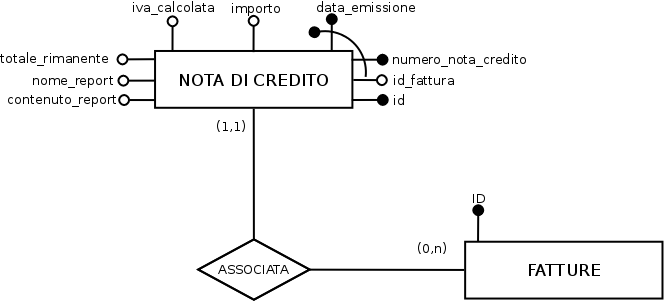
\includegraphics[scale=0.5]{img/schema_concettuale}
\newline
Sono state attuate le seguenti scelte sugli attributi:
\begin{enumerate}
    \item L' attributo \texttt{totale\_rimanente} anche se attributo 
        derivato viene comunque messo per velocizzare le operazioni di 
        visualizzazione delle fatture in modo che non si debba fare ogni volta 
        i calcoli dell’ imponibile con le note di credito.
    \item Sono presenti due chiavi, la prima, chiave primaria, è un \texttt{id} 
        numerico auto incrementante mentre la seconda, chiave canditata, è 
        data dalla coppia \texttt{numero\_nota\_credito} e 
        \texttt{data\_emissione}.
        L'attributo \texttt{id\_fattura} è una chiave esterna ed è associata 
        con l'attributo \texttt{id} che è chiave dell' entità fattura.
    \item Abbiamo due attributi, \texttt{nome\_report} e 
        \texttt{contenuto\_report}, che contegono il nome e il contenuto 
        del file \texttt{.pdf} della nota di credito appena generata.
    \item Sono stati inseriti inoltre solo l’importo e l’ IVA calcolata in 
        quanto la percentuale dell’ IVA utilizzata e l’importo totale della 
        nota di credito possono essere ricavate dagli attributi importo e 
        IVA calcolata.
\end{enumerate}
\subsection{Schema Logico}
Si è quindi passato poi allo schema logico ricavato da quello concettuale.
\newline
\newline
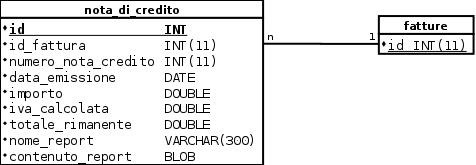
\includegraphics[scale=0.5]{img/schema_logico}
\newline
Come numero di cifre intere è stato scelto undici per rimanere in linea con il
numero di cifre dell' id della tabella \texttt{fattura}
\subsection{Codice SQL}
Il codice della tabella in SQL è il seguente
\lstinputlisting[basicstyle=\ttfamily\scriptsize,title=Codice SQL della tabella]{code/tabella.sql}
Per tutti i campi è stato deciso di renderli tutti non nulli perché alla
generazione della nota di credito tutti i campi devono essere compilati.
\section{Implementazione della funzionalità}
Si è passati poi alla scrittura del codice per integrare la nuova funzionalità
nell' applicativo.
Per questa parte sono stato aiutato da due sviluppatori interni all' azienda
di nome Mauro Veronese della sede di Padova e Rocco Spenza della sede di Roma.
\subsection{Bean delle note di credito}
Come prima cosa dopo la creazione del database si è dovuto scrivere il Bean per 
poter mappare la tabella in Hibernate.
\lstinputlisting[basicstyle=\ttfamily\scriptsize,firstline=22,lastline=64,title=Bean della tabella delle note di credito]{code/bean/NotaDiCredito.java}
Si è scelto inoltre di indicare tramite le notazioni Java di effettuare un Join
automatico con la tabella delle fatture essendo che nella maggioranza delle 
operazioni era necessario avere anche i dati della fattura associata.
\subsection{Lista delle fatture}
Successivamente si è passato a modificare la lista di visualizzazione delle 
fatture fatta precedentemente 
integrando l' inserimento delle note di credito all' interno dell' interfaccia 
di inserimento fatture.
\newline
\newline
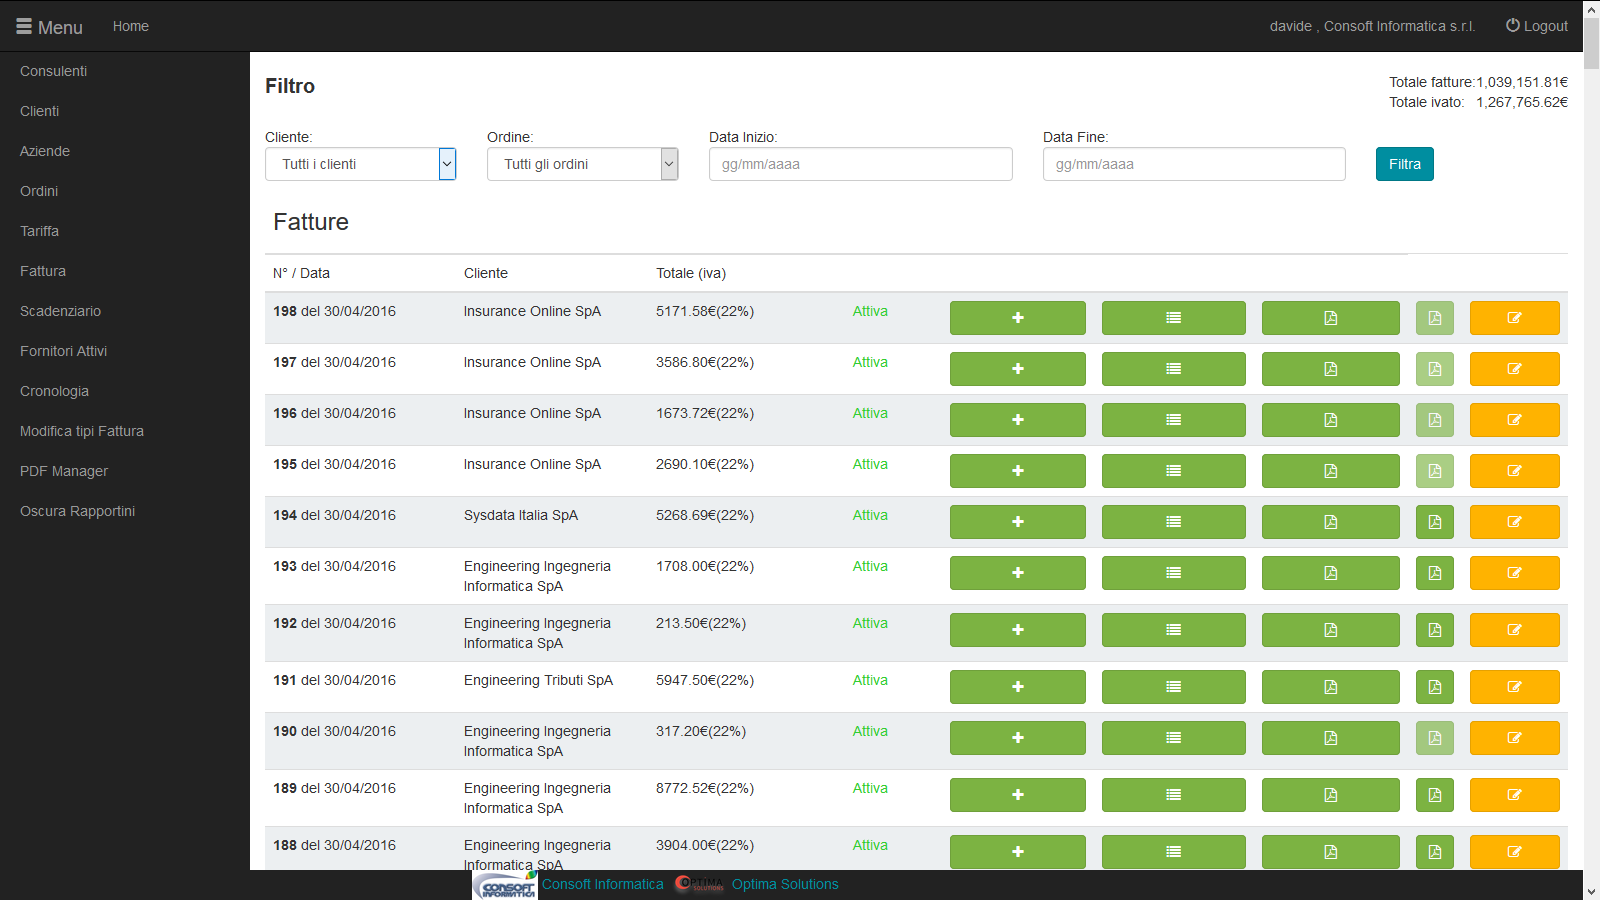
\includegraphics[scale=0.4]{img/lista_fatture}
\newline
Sono stati inseriti i due bottoni verdi \includegraphics[scale=0.4]{img/add} e 
\includegraphics[scale=0.4]{img/list} i quali sono rispettivamente per l' inserimento e 
la visualizzazione della nota di credito per ogni fattura.
\subsection{Inserimento e modifica della nota di credito}
In seguito abbiamo cominciato a costruire l' interfaccia per l' inserimento 
e la modifica di una nota di credito.
Si è reso indispensabile per una interfaccia coerente con entrambe le operazioni
di utilizzare una sola pagina web.
Per determinare il tipo di pagina si è deciso di verificare dentro alla pagina
jsp, attraverso il valore di un attributo dentro alla web request, per poter poi 
inviare la form alla funzione del controller più adatta.
\lstinputlisting[firstline=8,lastline=14,basicstyle=\ttfamily\scriptsize,title=Codice per la decisione dell' azione da compiere]{code/view/inserimentoModificaNoteCredito.jsp}
La pagina web di inserimento finita si presenta così.
\newline
\newline
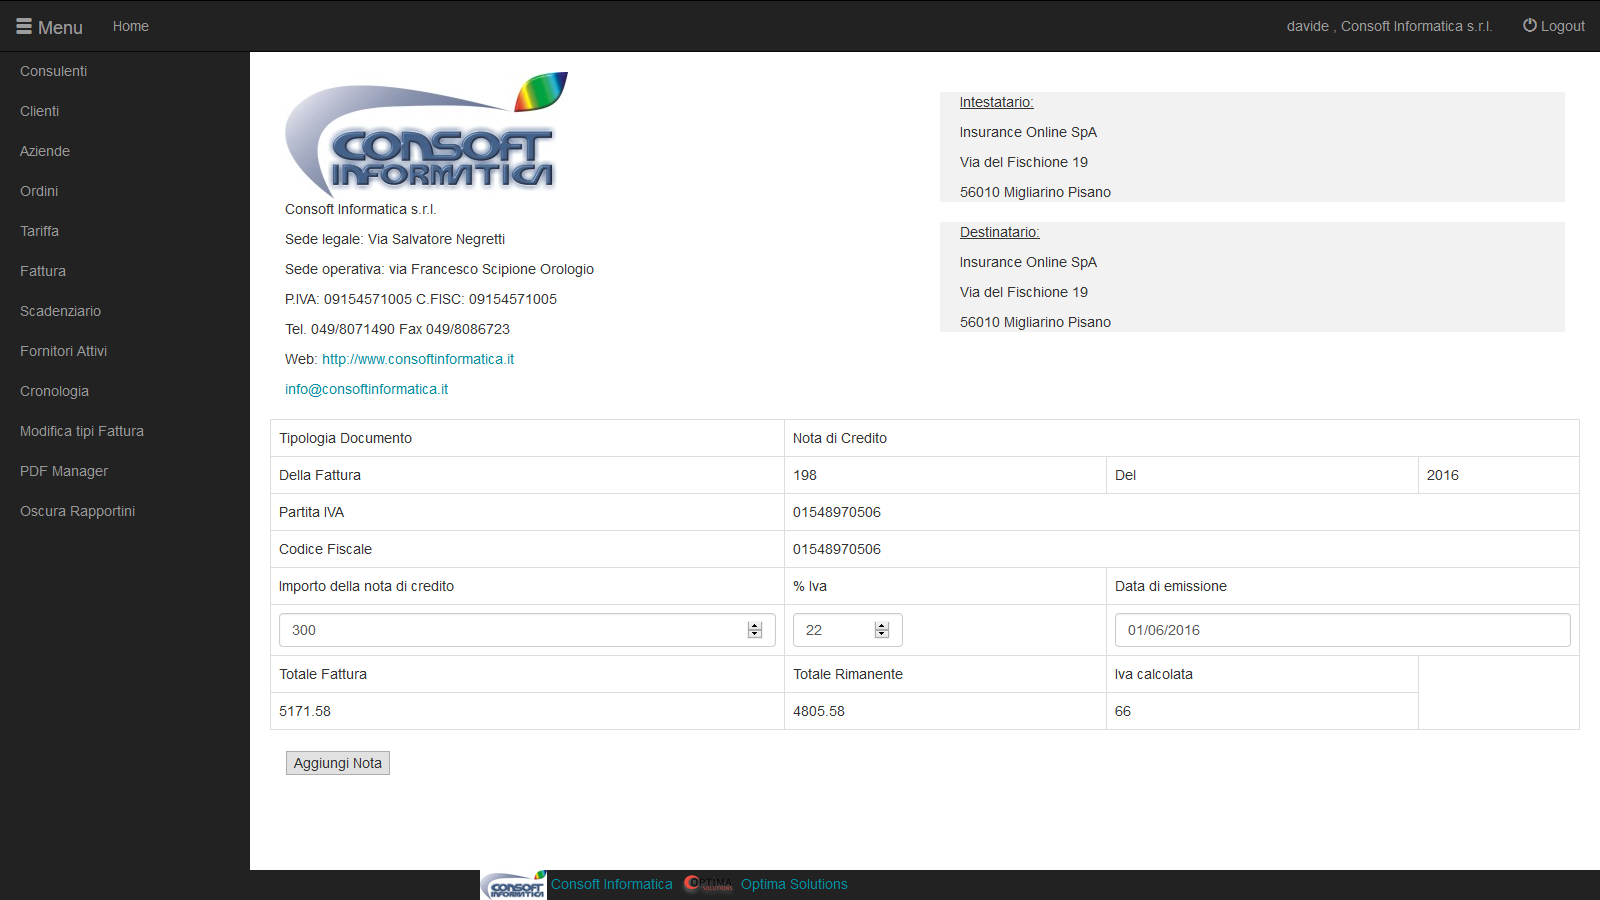
\includegraphics[scale=0.4]{img/inserimento_nota_credito}
\newline
La cui struttura è data dal seguente codice html.
\lstinputlisting[firstline=100,lastline=172,basicstyle=\ttfamily\scriptsize,title=Codice Html della parte frontend]{code/view/inserimentoModificaNoteCredito.jsp}
Dove \(\texttt{\$\{azione\}}\) indica il tipo di web request che deve essere
fatta alla sottomissione della form che viene determinata attraverso il 
codice visto precedentemente.
Il calcolo del totale che verrà detratto viene fatto 
con codice \texttt{Javascript/jQuery} che esegue i calcoli ogni 
volta che l'importo o l' iva viene modificato come si può vedere qui sotto.
\lstinputlisting[firstline=175,lastline=190,basicstyle=\ttfamily\scriptsize,title=Codice javascript per la parte frontend]{code/view/inserimentoModificaNoteCredito.jsp}
\subsubsection{Inserimento}
Prima dell' inserimento dei dati nel database tutti i calcoli però vengono 
fatti anche in Java dentro al controller per evitare manomissioni 
nell' inserimento semplicemente modificando l'\texttt{html}.
Inoltre per si utilizza una funzione di Spring per la validazione dei dati.
Consiste nell' associare al form di inserimento un oggetto di una classe simile
ad un Bean con delle notazioni Java che verificano se i parametri inviati 
corrispondono al dominio richiesto. La classe è stata chiamata 
\texttt{NotaCreditoForm} e la sua implementazione è qui sotto.
\lstinputlisting[firstline=16,lastline=33,basicstyle=\ttfamily\scriptsize,title=form di controllo delle note di credito]{code/form/NotaCreditoForm.java}
Per poter procedere alla vera e propria validazione bisogna, all'interno della
funzione del controller che riceve i dati, specificare all' interno dei 
parametri il nome dell' oggetto da validare e un oggetto di tipo 
\texttt{BindingResult} già implementato Spring e che procede materialmente alla
validazione tramite il metodo booleano \texttt{hasErrors}.
Nel caso in cui la validazione presenti degli errori verranno caricati 
nell' oggetto model i messaggi di errore all' interno delle notazioni nella 
classe di validazione e che verranno automaticamente visualizzati dentro ai
tag \texttt{form:errors} per ogni attributo in cui è stato trovato un errore.
La fase di controlli è scritta in questo listato di codice.
\lstinputlisting[firstline=257,lastline=293,basicstyle=\ttfamily\scriptsize,title=parte di reperimento dati e controllo del controller delle note di credito]{code/controller/NotaCreditoController.java}
Infine, se tutti i controlli vanno a buon fine, avviene la creazione della nota di 
credito in formato \texttt{pdf} e il caricamento di tutti i dati nel database.
\lstinputlisting[firstline=342,lastline=375,basicstyle=\ttfamily\scriptsize,title=generazione del pdf e caricamento di tutti i dati]{code/controller/NotaCreditoController.java}
\subsubsection{Modifica}
Per la parte di modifica è necessario prima di tutto caricare i dati esistenti
dato l'id della nota di credito da modificare.
\lstinputlisting[firstline=192,lastline=214,breaklines=True,basicstyle=\ttfamily\scriptsize,title=Codice per il caricamento dei dati della nota di credito]{code/controller/NotaCreditoController.java}
Il caricamento dei dati viene fatto utilizzando la classe 
\texttt{NotaCreditoForm} usata nella fase di inserimento per la validazione.
Poi dopo aver effettuato le modifiche si usa la stessa procedura che abbiamo
visto nella fase di inserimento della nuova nota di credito.
\subsection{Lista delle note di credito}
Dopo l' inserimento e la modifica si è poi passati a scrivere la pagina jsp
che serve per visualizzare le note di credito precedentemente inserite.
La lista delle note di credito relativa ad una fattura può essere visualizzata
in due modi:
\begin{enumerate}
    \item Attraverso la pressione del tasto \includegraphics[scale=0.4]{img/list}
         nella lista delle fatture.
    \item Appena finito di compilare e salvare nel database una nota di credito.
\end{enumerate}
Un esempio di lista delle note di credito è la seguente immagine
\newline
\newline
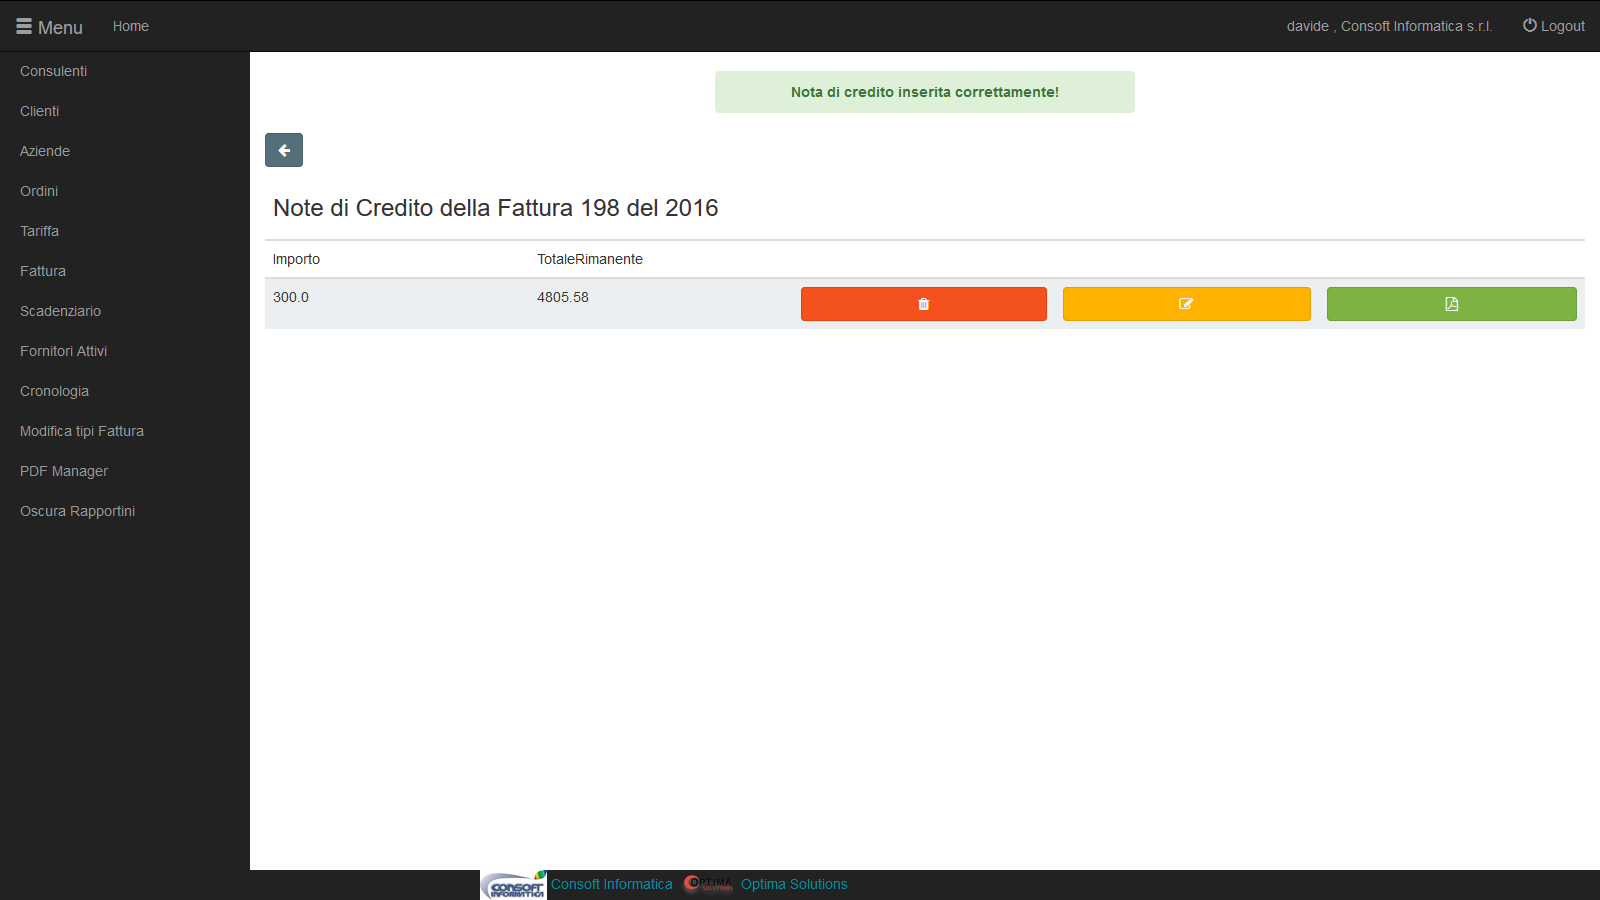
\includegraphics[scale=0.4]{img/visualizzazione_note_credito}
\newline
che viene generata dalla seguente parte di codice della pagina \texttt{visualizzeTutte.jsp}
La modifica e/o la cancellazione delle note di credito viene verificata 
grazie all' attributo modificabile e cancellabile che rappresenta l' id della
nota di credito al quale è associata tale azione.\lstinputlisting[basicstyle=\ttfamily\scriptsize,firstline=53,lastline=88,breaklines=True,title=Parte front end per la visualizzazione delle note di credito]{code/view/visualizzaTutte.jsp}
La parte del controller è piuttosto semplice infatti, dato l'id della fattura,
vengono ritornate tutte le sue note di credito compresi gli id della nota di 
credito che può essere modificata e/o cancellata.
\lstinputlisting[firstline=114,lastline=139,breaklines=True,basicstyle=\ttfamily\scriptsize,title=Funzione del controller per ritornare la lista delle note di credito.]{code/controller/NotaCreditoController.java}
\subsection{Eliminazione della nota di credito}
Dopodiché si è passati alla funzione di eliminazione della nota di credito.
Per l'eliminazione nel controller, dopo aver premuto il tasto di cancellazione, 
si cancella dal database la nota selezionata e viene
visualizzata nuovamente la lista delle rimanenti note di credito.
%TODO insert code
Nel caso in cui non ci siano note da mostrare la pagina avrà il seguente 
messaggio per comunicare che non ci sono note credito presenti.
\newline
\newline
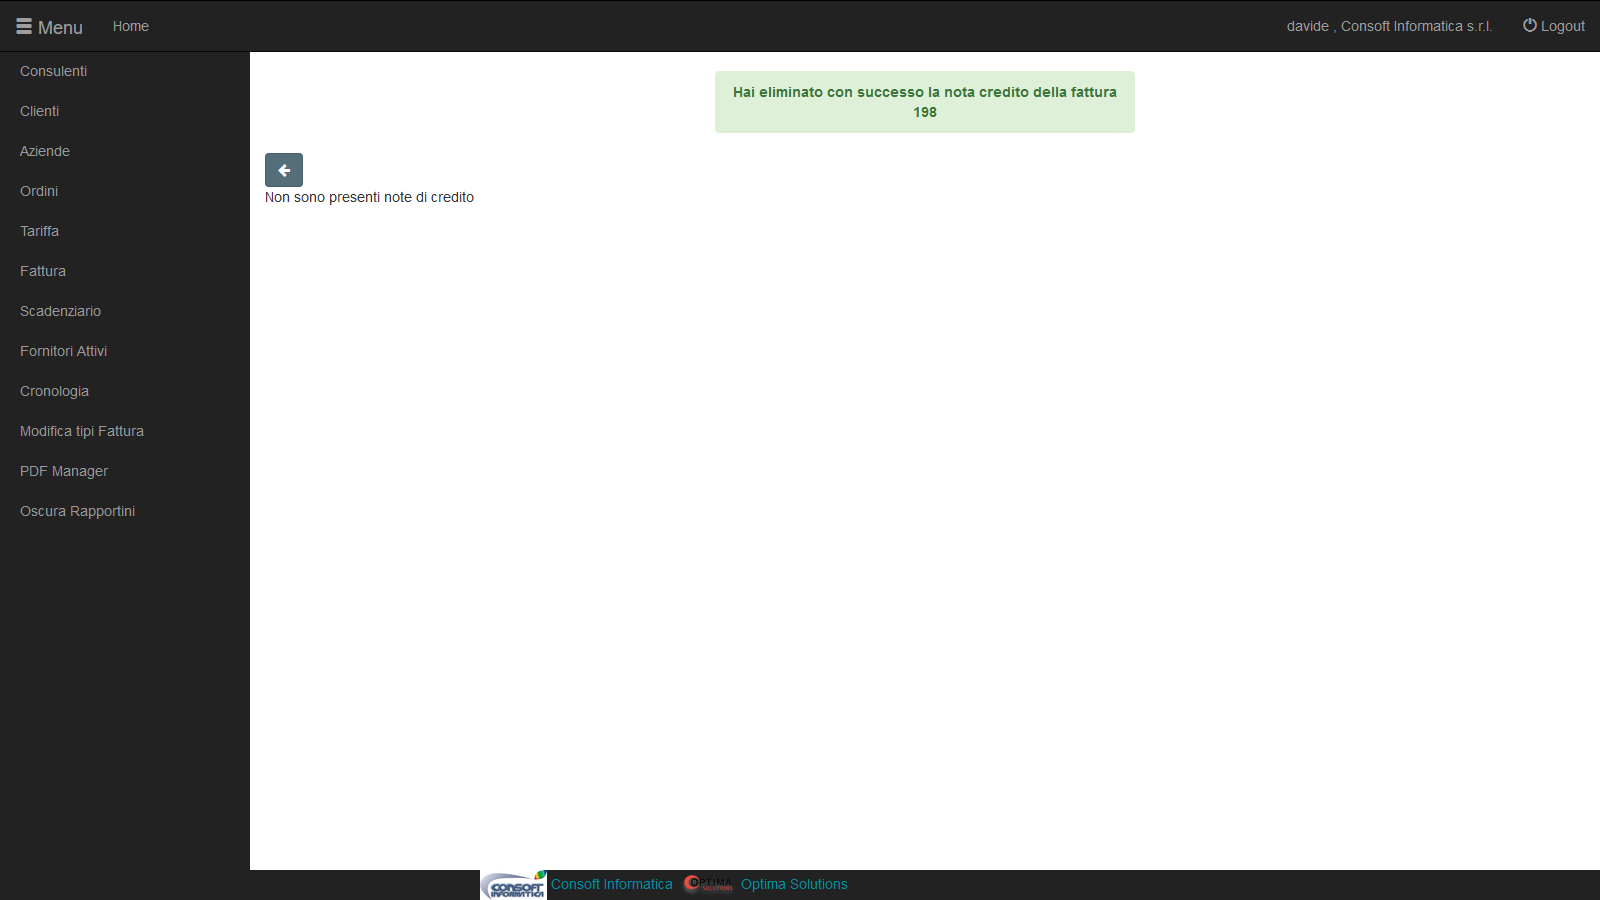
\includegraphics[scale=0.4]{img/eliminazione_nota_credito}
\newline
\subsection{Visualizzazione del pdf della nota di credito}
Infine per la visualizzazione della nota di credito viene generata, nel 
caso di un report non nullo, una response http di un documento in pdf
settando nell' header di risposta il tipo di documento (in questo caso pdf),
il nome del file ed infine il contenuto del file che viene inviato utilizzando
la classe \texttt{OutputStream} per poter inviare i byte del file attraverso 
lo stream di risposta.
%TODO insert code
Un esempio di nota di credito generate lo possiamo vedere nell' immagine 
qui sotto.
\chapter{Conclusione del lavoro e commenti finali}
Terminato lo sviluppo e dopo aver testato tutto nell' ambiente di prova tutto 
il lavoro svolto è stato caricato sul server di produzione senza la presenza
di problemi in fase di post produzione.
Durante tutto il lavoro io e gli altri due sviluppatori abbiamo collaborato 
attivamente tra di noi e con la nostra responsabile di progetto che, anche
se non era presente fisicamente per motivi di lavoro, è stata sempre presente
da remoto e ha sempre risposto ai nostri dubbi.
Tutto il tirocinio si è svolto senza problemi e le persone con cui ho avuto 
il piacere di collaborare durante il mio periodo in azienda sono stati sempre
cordiali e disponibili in ogni situazione.
\begin{thebibliography}{9}
    \bibitem{consoft:descrizione} Sito ufficiale Consoft Informatica \newline
    \texttt{http://www.consoftinformatica.it}
    \bibitem{apress:introducing_spring_framework}Felipe Gutierrez, 
    \emph{Introducing Spring Framework: A Primer}, Apress.
    \newline
\end{thebibliography}
\end{document}
